The \textit{Repository Management} module is responsible for management and cataloging of
algorithms and test data to be used in the benchmarking tests.

\subsection{Domain Model}
The domain model for the Repository Management module is shown in Figure \ref{fig:repoManDomain}
\begin{figure}[H]
  \begin{center}
  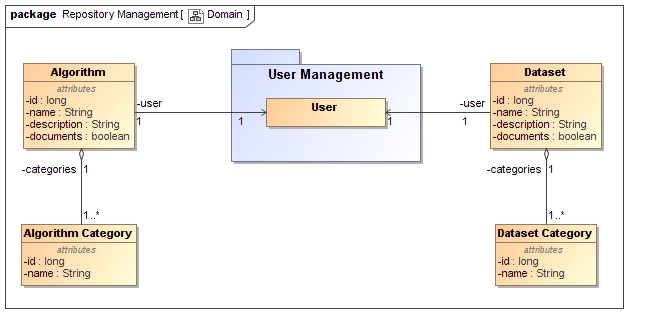
\includegraphics[scale=0.38]{../Diagrams and Charts/Repository Management/Domain.jpg}  
  \caption{Repository Management Domain Model}
  \label{fig:repoManDomain}
  \end{center}  
\end{figure}



\subsection{Scope}
The scope for the Repository Management module is complex because of the 
constraints placed upon the use cases by the business requirements. Therefore
the module scope has been broken down into different levels of granularity to
clarify the business requirements. A high level overview of the scope is given in
Figure \ref{fig:repositoryManagementHighLevelScope}
\begin{figure}[H]
  \begin{center}
  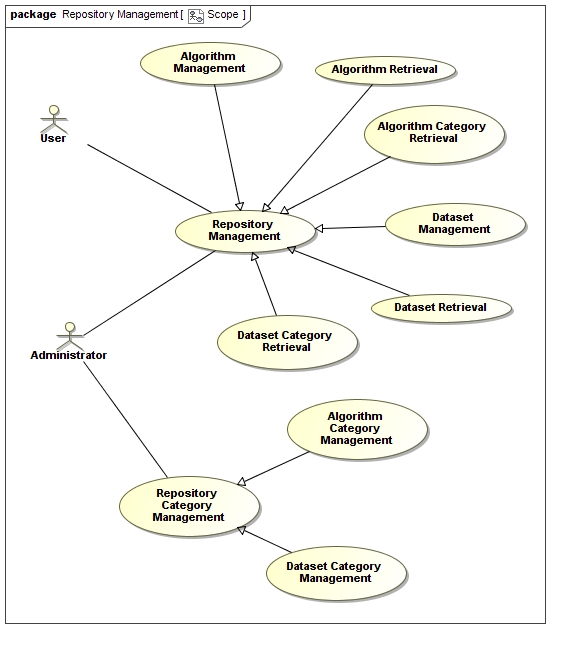
\includegraphics[scale=0.38]{../Diagrams and Charts/Repository Management/Scope.jpg}
  \caption{High Level Scope overview of Repository Management}
  \label{fig:repositoryManagementHighLevelScope}
  \end{center}  
\end{figure}

For the dataset use cases four major scopes have been identified:
\begin{itemize}
  \item Dataset Management
  \item Dataset Retrieval
  \item Dataset Category Management
  \item Dataset Category Retrieval
\end{itemize}



\subsubsection{Dataset Management}
The dataset management scope is concerned with all responsibilities related to
the CRUD management of datasets in the repository. Important to note, that the
dataset it self can't be updated, but only the metadata associated with a 
dataset can be updated. This is done to ensure consistency in the system, as it
was stated by a client, that any modification to a dataset constitutes a new 
entity.
\begin{figure}[H]
  \begin{center}
  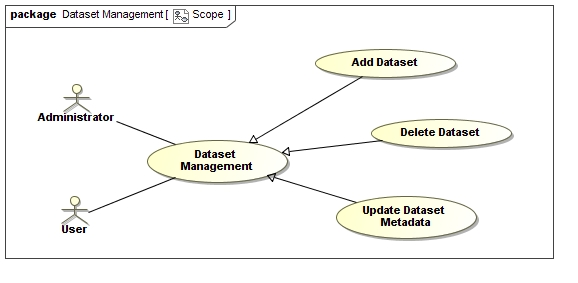
\includegraphics[scale=0.38]{../Diagrams and Charts/Repository Management/Dataset Management Scope.jpg}
  \caption{Scope overview of Dataset Management}
  \end{center}  
\end{figure}

\subsubsection{Dataset Retrieval}
This scope details the various retrieval mechanism by which datasets can be 
retrieved.
\begin{figure}[H]
  \begin{center}
  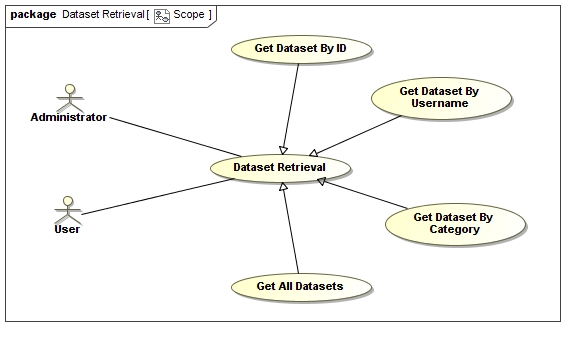
\includegraphics[scale=0.38]{../Diagrams and Charts/Repository Management/Dataset Retrieval Scope.jpg}
  \caption{Scope overview of Dataset Retrieval}
  \end{center}  
\end{figure}

\subsubsection{Dataset Category Management}
The CRUD management of dataset classifiers is limited only to administrator
users as the client want to prevent the pollution of the system with user
created categories.
\begin{figure}[H]
  \begin{center}
  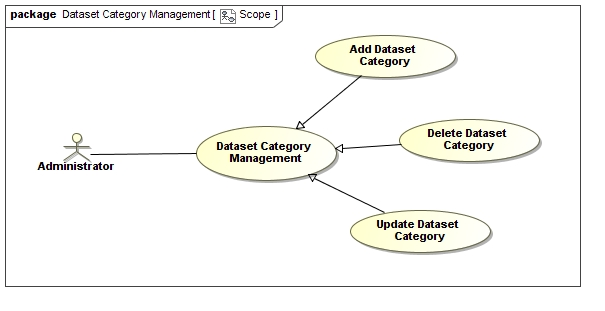
\includegraphics[scale=0.38]{../Diagrams and Charts/Repository Management/Dataset Category Management Scope.jpg}
  \caption{Scope overview of Dataset Category Management}
  \end{center}  
\end{figure}

\subsubsection{Dataset Category Retrieval}
This scope details the various retrieval mechanism by which dataset classifiers 
can be retrieved.
\begin{figure}[H]
  \begin{center}
  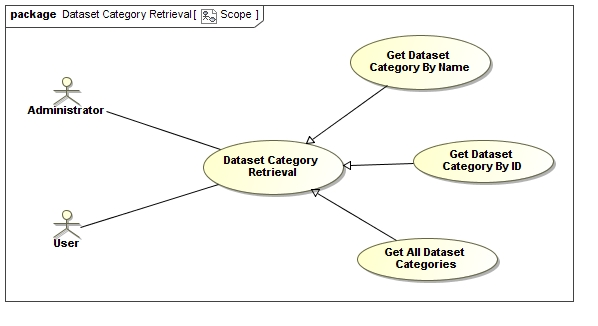
\includegraphics[scale=0.38]{../Diagrams and Charts/Repository Management/Dataset Category Retrieval Scope.jpg}
  \caption{Scope overview of Dataset Category Retrieval}
  \end{center}  
\end{figure}

\subsubsection{Algorithm and Algorithm Category Scope}
The algorithm and algorithm category scopes is mutatis mutandis the same as for
the dataset and dataset categories.



\subsection {Add Dataset}
The \textit{Add Dataset} use case is concerned with adding a user uploaded
dataset to the repository management system. This will allow the dataset to be
used in the creation of experiments.

\subsubsection{Service Contract}
The service contract for adding a dataset is shown in Figure \ref{fig:addDatasetService}
\begin{figure}[H]
  \begin{center}
  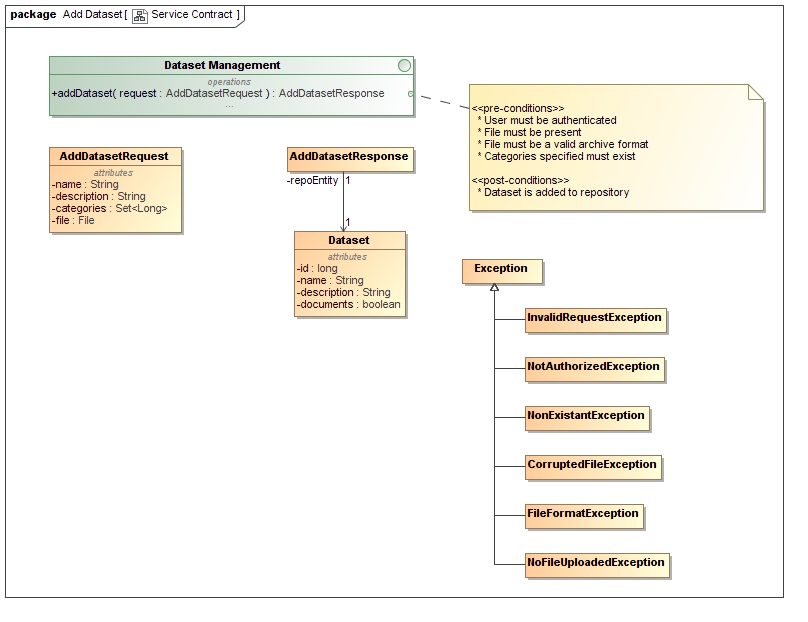
\includegraphics[scale=0.38]{../Diagrams and Charts/Repository Management/Add Dataset Service Contract.jpg}
  \caption{Add Dataset Service Contract}
  \label{fig:addDatasetService}
  \end{center}  
\end{figure}

The use case adds a user uploaded dataset to the management system. The
service is responsible for adding the metadata object to the relational
persistence provider and adding the uploaded archive to the document-based
persistence provider. Furthermore this use case is also responsible for
extracting the archive and storing each document in the document-based
persistence provider with a unique identifier, as to allow the user to request
individual documents from an uploaded archive.

\subsubsection{Functional Requirements}
The lower level services required by the add dataset service to either check the
pre-conditions or address the post-conditions are shown in Figure \ref{fig:addDatasetFR}
\begin{figure}[H]
  \begin{center}
  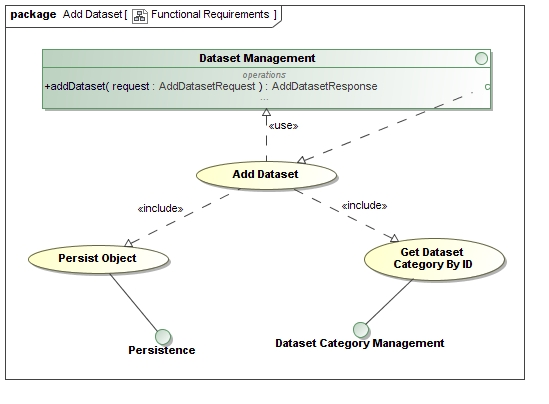
\includegraphics[scale=0.38]{../Diagrams and Charts/Repository Management/Add Dataset Functional Requirements.jpg}
  \caption{Add Dataset Functional Requirements}
  \label{fig:addDatasetFR}
  \end{center}
\end{figure}

\subsubsection{Process Design}
Refer to figure \ref{fig:addDatasetProcessDesign} on the process flow to add
a new user uploaded dataset to the benchmarking system. Note that the Get user
With Authorities and Get Dataset Category By ID are all responsible for checking
whether the obejct exists.
\begin{figure}[H]
  \begin{center}
  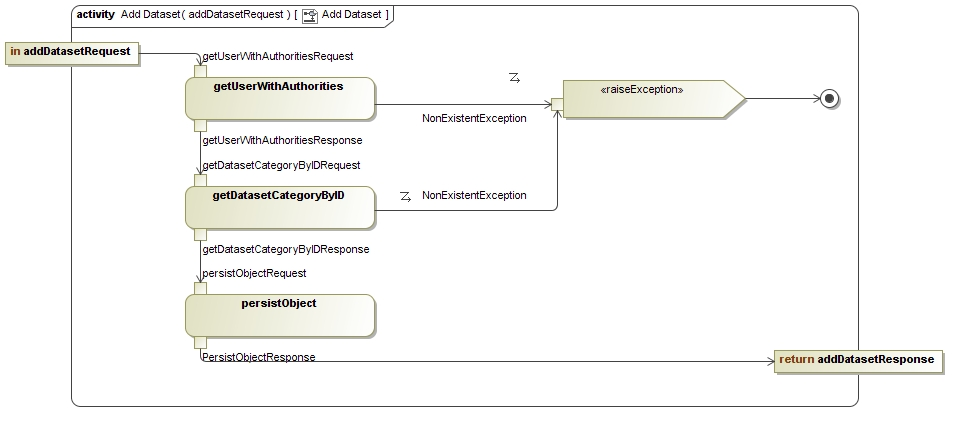
\includegraphics[scale=0.38]{../Diagrams and Charts/Repository Management/Add Dataset Process Design.jpg}
  \caption{Add Dataset Process Design}
  \label{fig:addDatasetProcessDesign}
  \end{center}
\end{figure}




\subsection {Delete Dataset}
The \textit{Add Dataset} use case is concerned with removing a user uploaded
dataset from the repository management system, however a dataset can only be
removed if it has not yet been used in an experiment definition.

\subsubsection{Service Contract}
The service contract for deleting a dataset is shown in Figure \ref{fig:deleteDatasetService}

\begin{figure}[H]
  \begin{center}
  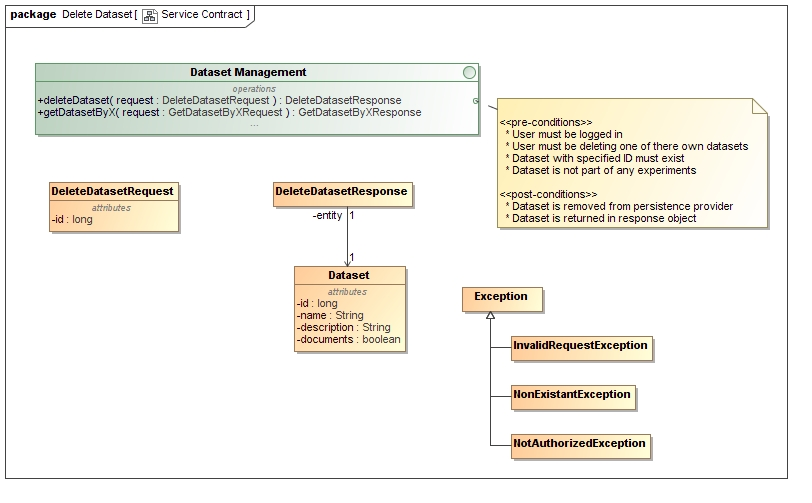
\includegraphics[scale=0.38]{../Diagrams and Charts/Repository Management/Delete Dataset Service Contract.jpg}
  \caption{Delete Dataset Service Contract}
  \label{fig:deleteDatasetService}
  \end{center}  
 \end{figure}

\subsubsection{Functional Requirements}
The lower level services required by the delete dataset service to either check the
pre-conditions or address the post-conditions are shown in Figure \ref{fig:deleteAlgorithmFuncReq}

\begin{figure}[H]
  \begin{center}
  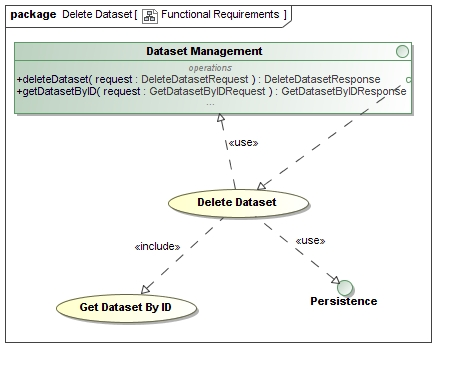
\includegraphics[scale=0.38]{../Diagrams and Charts/Repository Management/Delete Dataset Functional Requirements.jpg}
  \caption{Delete Dataset Functional Requirements}
  \label{fig:deleteAlgorithmFuncReq}
  \end{center}  
\end{figure}

\subsubsection{Process Design}
Refer to figure \ref{fig:deleteDatasetProcessDesign} on the process flow to delete
an uploaded dataset from the benchmarking system. Note that the Get user
With Authorities and Get Dataset Category By ID are all responsible for checking
whether the obejct exists. The Delete Dataset service is responsible for ensuring
that the user requesting the delete can only delete their own uploaded datasets.
\begin{figure}[H]
  \begin{center}
  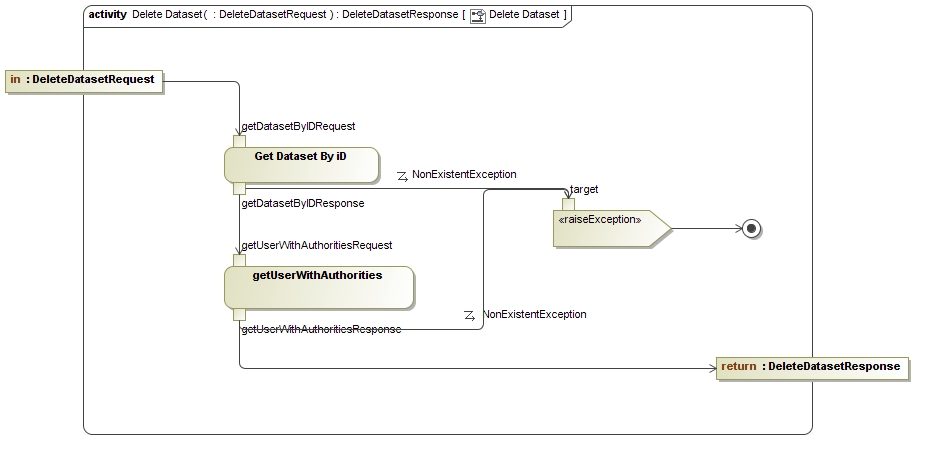
\includegraphics[scale=0.38]{../Diagrams and Charts/Repository Management/Delete Dataset Process Design.jpg}
  \caption{Delete Dataset Process Design}
  \label{fig:deleteDatasetProcessDesign}
  \end{center}
\end{figure}



\subsection {Update Dataset Metadata}
The \textit{Update Dataset Metadata} use case is concerned with updating the
metadata around a user uploaded dataset. Important to note that the actual
dataset may not and can not be updated, as this will violate the integrity of
results.
\subsubsection{Service Contract}
The service contract for updating a datasets metadata is shown in Figure \ref{fig:updateDatasetMetadataServiceContract}
\begin{figure}[H]
	\begin{center}
		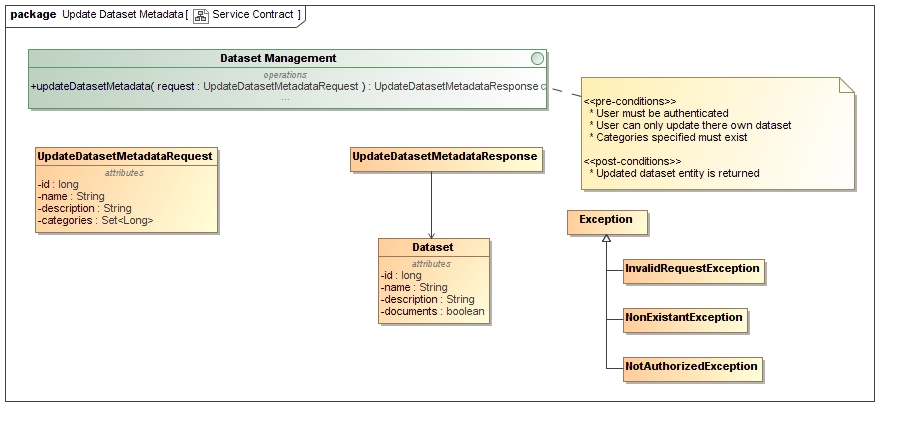
\includegraphics[scale=0.38]{../Diagrams and Charts/Repository Management/Update Dataset Metadata Service Contract.jpg}
		\caption{Update Dataset metadata Service Contract}
		\label{fig:updateDatasetMetadataServiceContract}
	\end{center}	
\end{figure}

\subsubsection{Functional Requirements}
The lower level services required by the update dataset metadata service to
either check the pre-conditions or address the post-conditions are shown in 
Figure \ref{fig:UpdateDatasetMetadataUseCase}
\begin{figure}[H]
	\begin{center}
		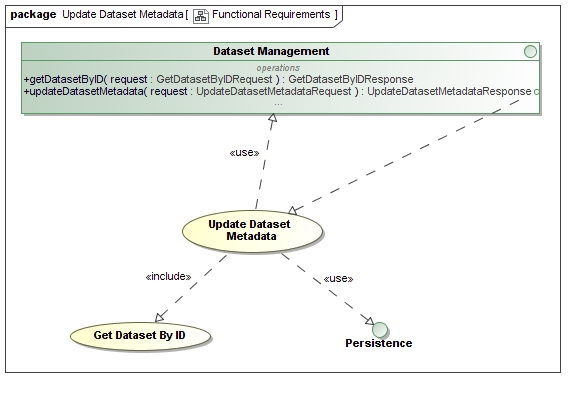
\includegraphics[scale=0.38]{../Diagrams and Charts/Repository Management/Update Dataset Metadata Functional Requirements.jpg}
		\caption{Update Dataset Metadata Functional Requirements}
		\label{fig:UpdateDatasetMetadataUseCase}
	\end{center}
\end{figure}



\subsection{Get Dataset By X}
3 similar use case have been defined to retrieve the dataset upon namely
\begin{itemize}
  \item Get Dataset By Category
  \item Get Dataset By ID
  \item Get Dataset By Username
\end{itemize}

All service contracts, functional requirements are implementations are mutatis 
mutandis the same, except the parameter which is filtered upon. The respective
request and response objects can be seen in figure \ref{fig:getDatasetByXServiceContract}.

\subsubsection{Service Contract}
The generic service contract for retrieving a dataset upon a parameter is show in
Figure \ref{fig:getDatasetByXServiceContract}
\begin{figure}[H]
  \begin{center}
  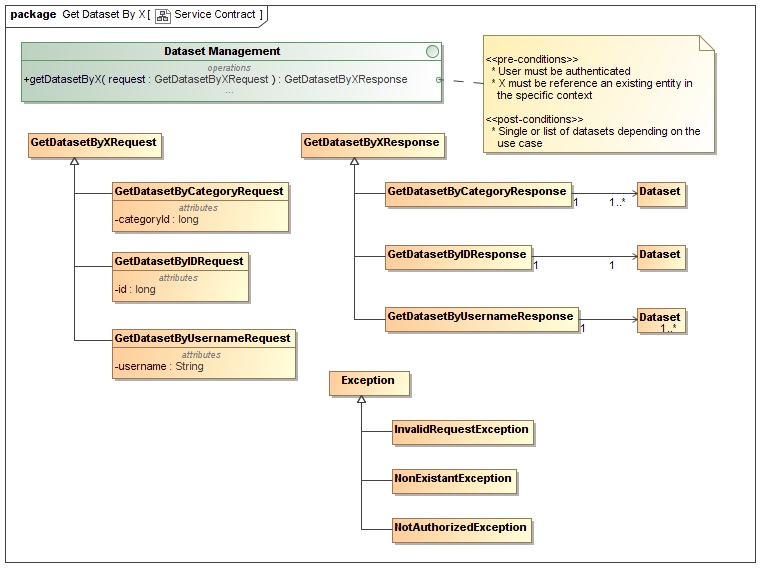
\includegraphics[scale=0.38]{../Diagrams and Charts/Repository Management/Get Dataset By X Service Contract.jpg}
  \caption{Get Dataset by X Service Contract}
  \label{fig:getDatasetByXServiceContract}
  \end{center}
\end{figure}

\subsubsection{Functional Requirements}
The lower level services required by the generic get dataset by X service
to either check the pre-conditions or address the post-conditions are shown in Figure 
\ref{fig:getDatasetByXFuncReq}
\begin{figure}[H]
  \begin{center}
  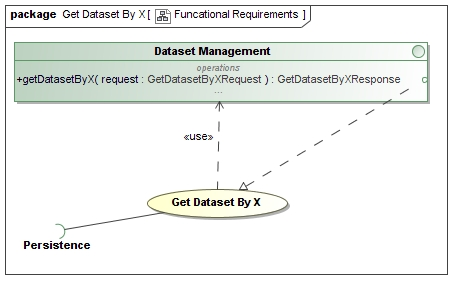
\includegraphics[scale=0.38]{../Diagrams and Charts/Repository Management/Get Dataset By X Funcational Requirements.jpg}
  \caption{Get Dataset by X Functional Requirements}
  \label{fig:getDatasetByXFuncReq}
  \end{center}
\end{figure}



\subsection {Get All Datasets}
The \textit{Get All Datasets} use case is concerned with retrieving all datasets
from the back end system.
\subsubsection{Service Contract}
The service contract for retrieving all datasets is shown in 
Figure \ref{fig:getAllDatasetsServiceContract}.
\begin{figure}[H]
  \begin{center}
  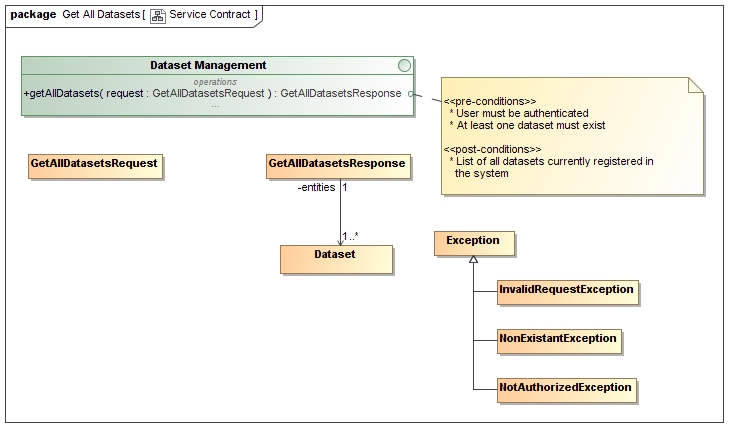
\includegraphics[scale=0.38]{../Diagrams and Charts/Repository Management/Get All Datasets Service Contract.jpg}
  \caption{Get All Datasets Service Contract}
  \label{fig:getAllDatasetsServiceContract}
  \end{center}
\end{figure}



\subsection{Algorithm Management}
The algorithm management service contract and implementation is mutatis mutandis
the same as that of the dataset management.



\subsection {Add Dataset Category}
The \textit{Add Dataset Category} use case is concerned with adding a new
dataset category that can be used to classify datasets. 

\subsubsection{Service Contract}
The service contract for adding a dataset category is shown in 
Figure \ref{fig:addDatasetCategoryServiceContract}.
\begin{figure}[H]
  \begin{center}
  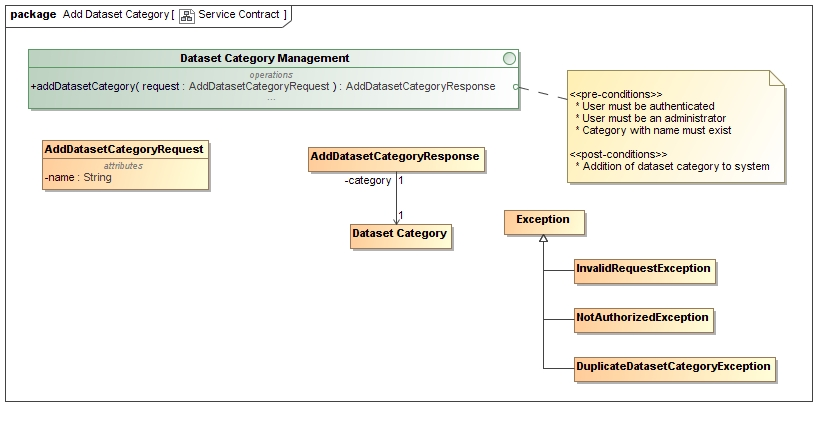
\includegraphics[scale=0.38]{../Diagrams and Charts/Repository Management/Add Dataset Category Service Contract.jpg}
  \caption{Add Dataset Category Service Contract}
  \label{fig:addDatasetCategoryServiceContract}
  \end{center}
\end{figure}

\subsubsection{Functional Requirements}
The lower level services required by the update dataset metadata service to
either check the pre-conditions or address the post-conditions are shown in 
Figure \ref{fig:addDatasetCategoryFunctionalRequirements}.
\begin{figure}[H]
  \begin{center}
  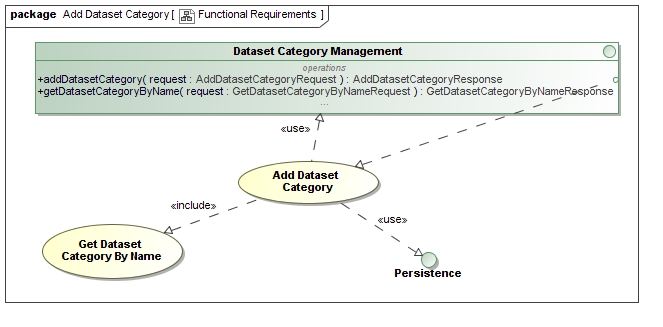
\includegraphics[scale=0.38]{../Diagrams and Charts/Repository Management/Add Dataset Category Functional Requirements.jpg}
  \caption{Add Dataset Category Service Contract}
  \label{fig:addDatasetCategoryFunctionalRequirements}
  \end{center}
\end{figure}



\subsection {Delete Dataset Category}
The \textit{Delete Dataset Category} use case is concerned with removing a
dataset category from the back end.

\subsubsection{Service Contract}
The service contract for deleting a dataset category is shown in 
Figure \ref{fig:deleteDatasetCategoryServiceContract}.
\begin{figure}[H]
  \begin{center}
  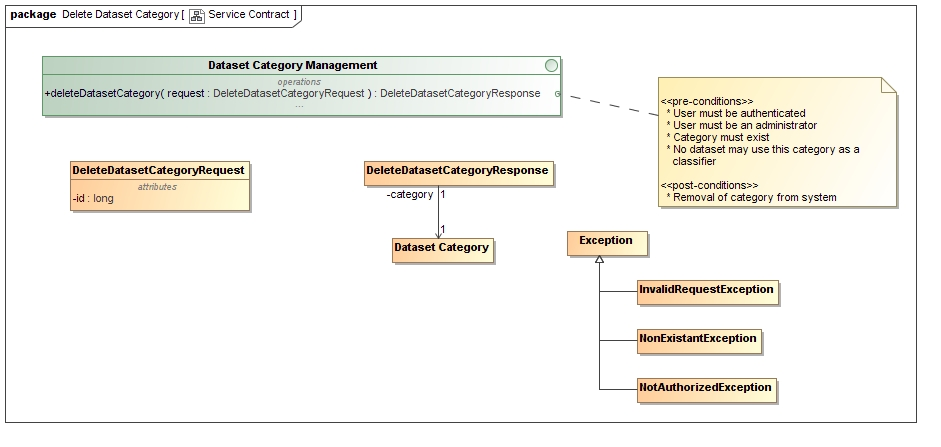
\includegraphics[scale=0.38]{../Diagrams and Charts/Repository Management/Delete Dataset Category Service Contract.jpg}
  \caption{Delete Dataset Category Service Contract}
  \label{fig:deleteDatasetCategoryServiceContract}
  \end{center}
\end{figure}



\subsection {Update Dataset Category}
The \textit{Update Dataset Category} use case is concerned with updating a
dataset category.

\subsubsection{Service Contract}
The service contract for updating a dataset category is shown in 
Figure \ref{fig:uupdateDatasetCategoryServiceContract}.
\begin{figure}[H]
  \begin{center}
  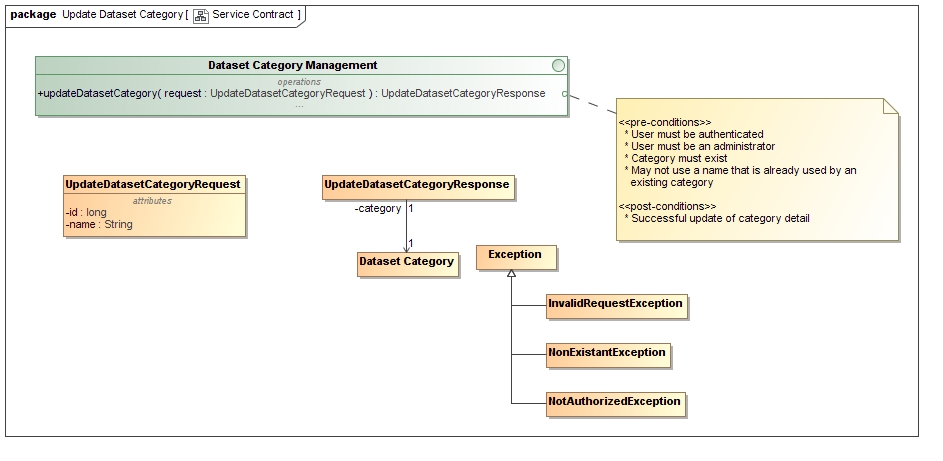
\includegraphics[scale=0.38]{../Diagrams and Charts/Repository Management/Update Dataset Category Service Contract.jpg}
  \caption{Update Dataset Category Service Contract}
  \label{fig:uupdateDatasetCategoryServiceContract}
  \end{center}
\end{figure}

\subsubsection{Functional Requirements}
The lower level services required by the update dataset metadata service to
either check the pre-conditions or address the post-conditions are shown in 
Figure \ref{fig:updateDatasetCategoryFunctionalRequirements}.
\begin{figure}[H]
  \begin{center}
  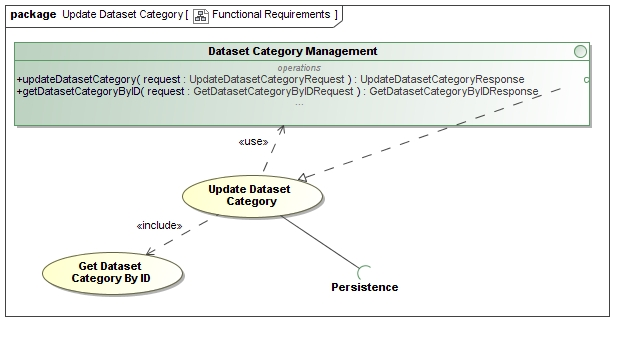
\includegraphics[scale=0.38]{../Diagrams and Charts/Repository Management/Update Dataset Category Functional Requirements.jpg}
  \caption{Update Dataset Category Service Contract}
  \label{fig:updateDatasetCategoryFunctionalRequirements}
  \end{center}
\end{figure}



\subsection {Get Dataset Category By X}
2 similar use case have been defined to retrieve the dataset category upon namely
\begin{itemize}
  \item Get Dataset Category By ID
  \item Get Dataset Category By Name
\end{itemize}

All service contracts, functional requirements are implementations are mutatis 
mutandis the same, except the parameter which is filtered upon. The respective
request and response objects can be seen in 
Figure \ref{fig:getDatasetCategoryByXServiceContract}.
\subsubsection{Service Contract}
\begin{figure}[H]
  \begin{center}
  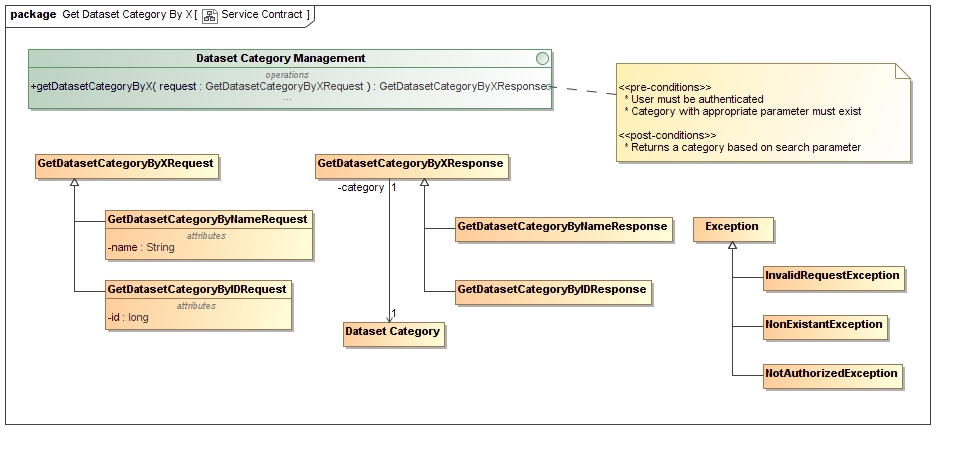
\includegraphics[scale=0.38]{../Diagrams and Charts/Repository Management/Get Dataset Category By X Service Contract.jpg}
  \caption{Get Dataset by X Service Contract}
  \label{fig:getDatasetCategoryByXServiceContract}
  \end{center}
\end{figure}

\subsubsection{Functional Requirements}
The lower level services required by the update dataset metadata service to
either check the pre-conditions or address the post-conditions are shown in 
Figure \ref{fig:getDatasetCategoryByXFunctionalRequirements}.
\begin{figure}[H]
  \begin{center}
  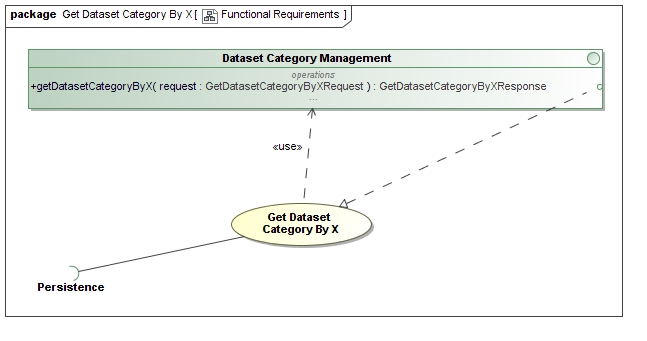
\includegraphics[scale=0.38]{../Diagrams and Charts/Repository Management/Get Dataset Category By X Functional Requirements.jpg}
  \caption{Get Dataset by X Functional Requirements}
  \label{fig:getDatasetCategoryByXFunctionalRequirements}
  \end{center}
\end{figure}



\subsection {Get All Dataset Categories}
The \textit{Get All Dataset Categories} use case is concerned with retrieving a
list of all dataset categories in the back end.

\subsubsection{Service Contract}
The service contract for getting all dataset categories is shown in 
Figure \ref{fig:getAllDatasetCategoriesServiceContract}.
\begin{figure}[H]
  \begin{center}
  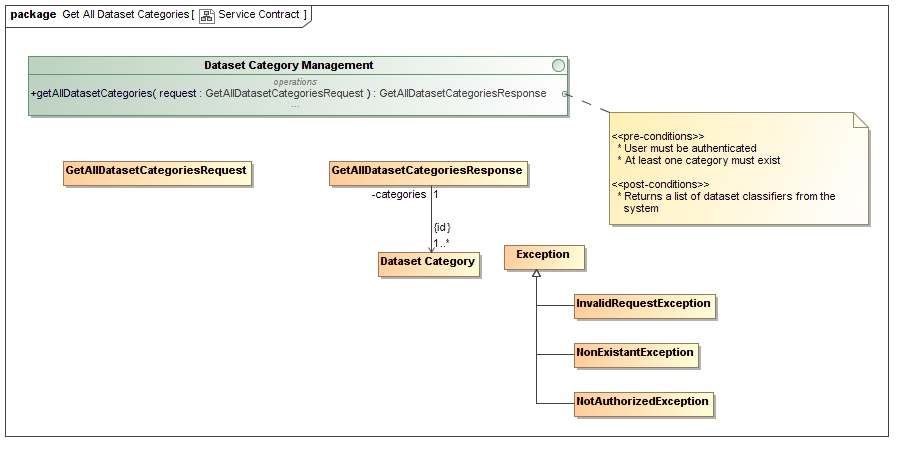
\includegraphics[scale=0.38]{../Diagrams and Charts/Repository Management/Get All Dataset Categories Service Contract.jpg}
  \caption{Get All Dataset Categories Service Contract}
  \label{fig:getAllDatasetCategoriesServiceContract}
  \end{center}
\end{figure}



\subsection{Algorithm Category Management}
The algorithm category management service contract and implementation is 
mutatis mutandis the same as that of the dataset category management.
